\documentclass[leqno, 12pt]{article}
\usepackage{tikz}
\usetikzlibrary{positioning}
\usetikzlibrary {arrows.meta}
\usetikzlibrary{bending}
\usepackage{ulem}
\usepackage[a4paper, portrait, margin=1cm]{geometry}
\usepackage{fancyhdr}

\def\jumpheight{10}
% % \def\qgap{\rule[-1pt]{1.0em}{.25pt}}
\def\qgap{\raisebox{-1pt}{\dotuline{\phantom{X}}}}

\def \HeadingAnswers {\section*{\Large Name: \underline{\hspace{8cm}} \hfill Date: \underline{\hspace{3cm}}} \vspace{-3mm}
{Number lines: Answers} \vspace{1pt}\hrule}

% raise footer with page number; no header
\fancypagestyle{myfancypagestyle}{
  \fancyhf{} % clear all header and footer fields
  \renewcommand{\headrulewidth}{0pt} % no rule under header
  \fancyfoot[C] {\thepage} \setlength{\footskip}{14.5pt} % raise page number allowed min 14.5pt
}
\pagestyle{myfancypagestyle}  % apply myfancypagestyle

\begin{document}
  \HeadingAnswers
  \vspace{-1mm}
  \begin{equation}
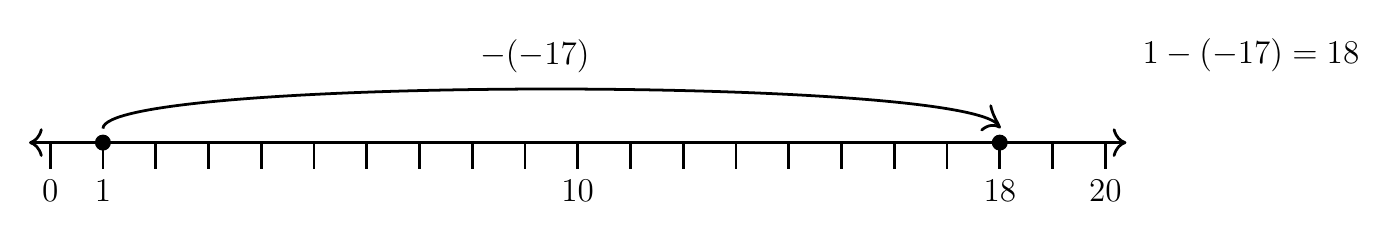
\begin{tikzpicture}[scale=0.67, baseline={([yshift=-1pt]current bounding box.north)}]
    % axis, arrow style to-to
    \draw[{To[scale=1.3]}-{To[scale=1.3]}, line width=1pt] (-0.4, 0) -- (20.4, 0);
    % tick marks
    \foreach \x in {0,1,...,20}
        \draw[shift={(\x,0)},color=black, line width=1pt] (0pt,-14pt) -- (0pt,0pt);
    % numbers along each axis
    \foreach \x in  {0,10,20}
        \draw[shift={(\x,-0.8)},color=black] node[font=\large,text height=12pt] {$\x$};
    \draw[shift={(1,-0.8)},color=black] node[font=\large,text height=12pt] {$1$};
    \draw[shift={(18,-0.8)},color=black] node[font=\large,text height=12pt] {$18$};
    % dots
    \filldraw[black] (1,0) circle (4pt) node[above,yshift=-2pt] (a) {};
    \filldraw[black] (18,0) circle (4pt) node[above,yshift=-2pt] (b) {};
    % arrow
    \draw[-{To[scale=1.3, bend]},line width=1pt, color=black] (a.north)  .. controls  +(north:\jumpheight mm) and +(north:\jumpheight mm) .. node[above=2pt,xshift=-6pt,font=\large,text height=10pt] {$-(-17)$} (b.north); % for addition
    % equation at right end
    \node [font=\large, anchor=east] at (25.0,1.65) {$1-(-17) = 18$};
\end{tikzpicture}
\end{equation}
\vspace{-2pt}\begin{equation}
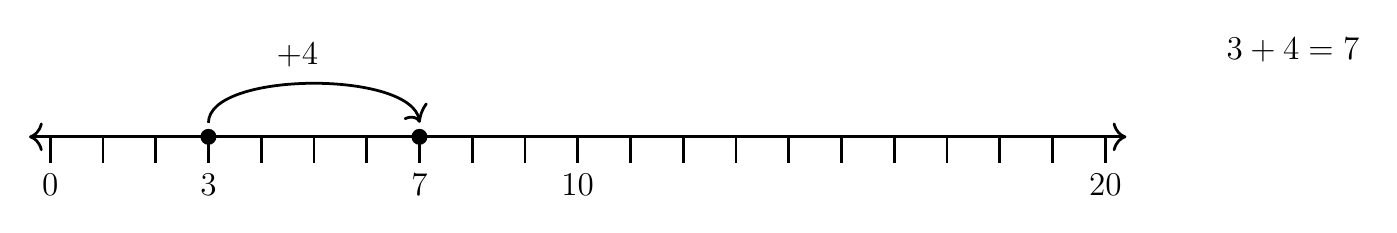
\begin{tikzpicture}[scale=0.67, baseline={([yshift=-1pt]current bounding box.north)}]
    % axis, arrow style to-to
    \draw[{To[scale=1.3]}-{To[scale=1.3]}, line width=1pt] (-0.4, 0) -- (20.4, 0);
    % tick marks
    \foreach \x in {0,1,...,20}
        \draw[shift={(\x,0)},color=black, line width=1pt] (0pt,-14pt) -- (0pt,0pt);
    % numbers along each axis
    \foreach \x in  {0,10,20}
        \draw[shift={(\x,-0.8)},color=black] node[font=\large,text height=12pt] {$\x$};
    \draw[shift={(3,-0.8)},color=black] node[font=\large,text height=12pt] {$3$};
    \draw[shift={(7,-0.8)},color=black] node[font=\large,text height=12pt] {$7$};
    % dots
    \filldraw[black] (3,0) circle (4pt) node[above,yshift=-2pt] (a) {};
    \filldraw[black] (7,0) circle (4pt) node[above,yshift=-2pt] (b) {};
    % arrow
    \draw[-{To[scale=1.3, bend]},line width=1pt, color=black] (a.north)  .. controls  +(north:\jumpheight mm) and +(north:\jumpheight mm) .. node[above=2pt,xshift=-6pt,font=\large,text height=10pt] {$+4$} (b.north); % for addition
    % equation at right end
    \node [font=\large, anchor=east] at (25.0,1.65) {$3+4 = 7$};
\end{tikzpicture}
\end{equation}
\vspace{-2pt}\begin{equation}
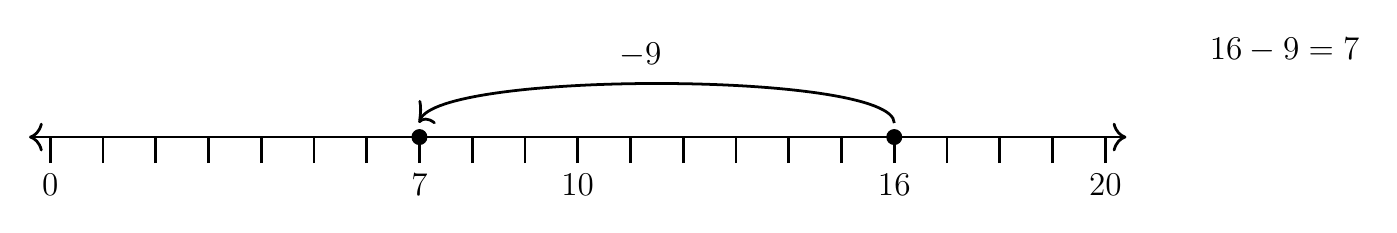
\begin{tikzpicture}[scale=0.67, baseline={([yshift=-1pt]current bounding box.north)}]
    % axis, arrow style to-to
    \draw[{To[scale=1.3]}-{To[scale=1.3]}, line width=1pt] (-0.4, 0) -- (20.4, 0);
    % tick marks
    \foreach \x in {0,1,...,20}
        \draw[shift={(\x,0)},color=black, line width=1pt] (0pt,-14pt) -- (0pt,0pt);
    % numbers along each axis
    \foreach \x in  {0,10,20}
        \draw[shift={(\x,-0.8)},color=black] node[font=\large,text height=12pt] {$\x$};
    \draw[shift={(16,-0.8)},color=black] node[font=\large,text height=12pt] {$16$};
    \draw[shift={(7,-0.8)},color=black] node[font=\large,text height=12pt] {$7$};
    % dots
    \filldraw[black] (16,0) circle (4pt) node[above,yshift=-2pt] (a) {};
    \filldraw[black] (7,0) circle (4pt) node[above,yshift=-2pt] (b) {};
    % arrow
    \draw[-{To[scale=1.3, bend]},line width=1pt, color=black] (a.north)  .. controls  +(north:\jumpheight mm) and +(north:\jumpheight mm) .. node[above=2pt,xshift=-6pt,font=\large,text height=10pt] {$-9$} (b.north); % for addition
    % equation at right end
    \node [font=\large, anchor=east] at (25.0,1.65) {$16-9 = 7$};
\end{tikzpicture}
\end{equation}
\vspace{-2pt}\begin{equation}
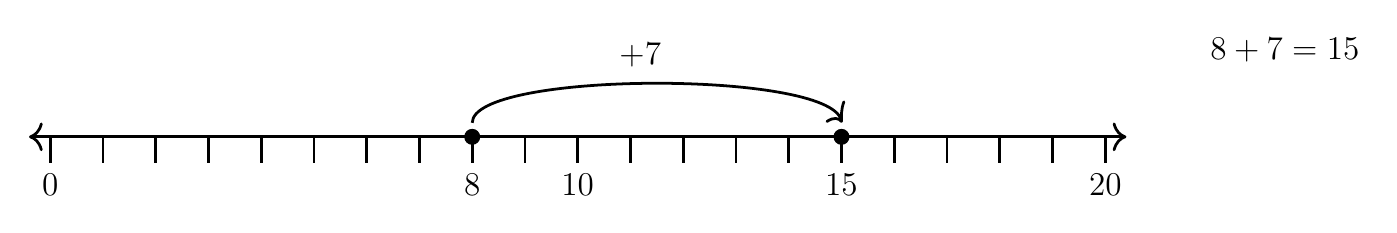
\begin{tikzpicture}[scale=0.67, baseline={([yshift=-1pt]current bounding box.north)}]
    % axis, arrow style to-to
    \draw[{To[scale=1.3]}-{To[scale=1.3]}, line width=1pt] (-0.4, 0) -- (20.4, 0);
    % tick marks
    \foreach \x in {0,1,...,20}
        \draw[shift={(\x,0)},color=black, line width=1pt] (0pt,-14pt) -- (0pt,0pt);
    % numbers along each axis
    \foreach \x in  {0,10,20}
        \draw[shift={(\x,-0.8)},color=black] node[font=\large,text height=12pt] {$\x$};
    \draw[shift={(8,-0.8)},color=black] node[font=\large,text height=12pt] {$8$};
    \draw[shift={(15,-0.8)},color=black] node[font=\large,text height=12pt] {$15$};
    % dots
    \filldraw[black] (8,0) circle (4pt) node[above,yshift=-2pt] (a) {};
    \filldraw[black] (15,0) circle (4pt) node[above,yshift=-2pt] (b) {};
    % arrow
    \draw[-{To[scale=1.3, bend]},line width=1pt, color=black] (a.north)  .. controls  +(north:\jumpheight mm) and +(north:\jumpheight mm) .. node[above=2pt,xshift=-6pt,font=\large,text height=10pt] {$+7$} (b.north); % for addition
    % equation at right end
    \node [font=\large, anchor=east] at (25.0,1.65) {$8+7 = 15$};
\end{tikzpicture}
\end{equation}
\vspace{-2pt}\begin{equation}
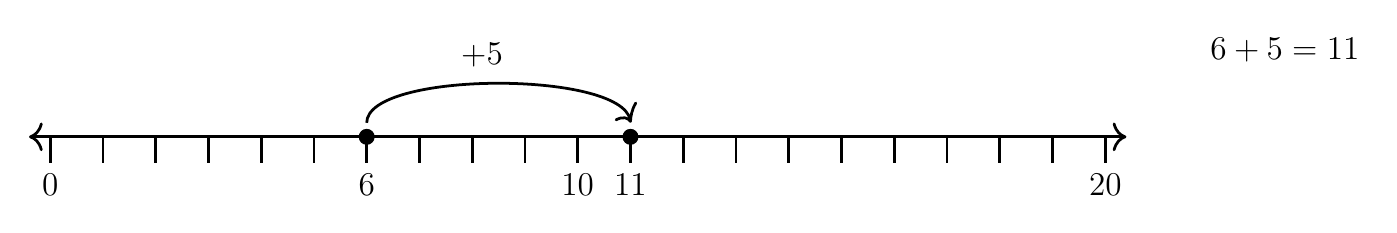
\begin{tikzpicture}[scale=0.67, baseline={([yshift=-1pt]current bounding box.north)}]
    % axis, arrow style to-to
    \draw[{To[scale=1.3]}-{To[scale=1.3]}, line width=1pt] (-0.4, 0) -- (20.4, 0);
    % tick marks
    \foreach \x in {0,1,...,20}
        \draw[shift={(\x,0)},color=black, line width=1pt] (0pt,-14pt) -- (0pt,0pt);
    % numbers along each axis
    \foreach \x in  {0,10,20}
        \draw[shift={(\x,-0.8)},color=black] node[font=\large,text height=12pt] {$\x$};
    \draw[shift={(6,-0.8)},color=black] node[font=\large,text height=12pt] {$6$};
    \draw[shift={(11,-0.8)},color=black] node[font=\large,text height=12pt] {$11$};
    % dots
    \filldraw[black] (6,0) circle (4pt) node[above,yshift=-2pt] (a) {};
    \filldraw[black] (11,0) circle (4pt) node[above,yshift=-2pt] (b) {};
    % arrow
    \draw[-{To[scale=1.3, bend]},line width=1pt, color=black] (a.north)  .. controls  +(north:\jumpheight mm) and +(north:\jumpheight mm) .. node[above=2pt,xshift=-6pt,font=\large,text height=10pt] {$+5$} (b.north); % for addition
    % equation at right end
    \node [font=\large, anchor=east] at (25.0,1.65) {$6+5 = 11$};
\end{tikzpicture}
\end{equation}
\vspace{-2pt}\begin{equation}
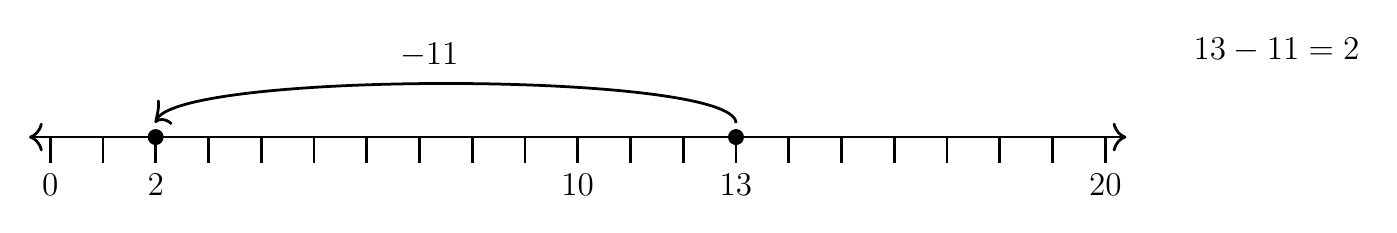
\begin{tikzpicture}[scale=0.67, baseline={([yshift=-1pt]current bounding box.north)}]
    % axis, arrow style to-to
    \draw[{To[scale=1.3]}-{To[scale=1.3]}, line width=1pt] (-0.4, 0) -- (20.4, 0);
    % tick marks
    \foreach \x in {0,1,...,20}
        \draw[shift={(\x,0)},color=black, line width=1pt] (0pt,-14pt) -- (0pt,0pt);
    % numbers along each axis
    \foreach \x in  {0,10,20}
        \draw[shift={(\x,-0.8)},color=black] node[font=\large,text height=12pt] {$\x$};
    \draw[shift={(13,-0.8)},color=black] node[font=\large,text height=12pt] {$13$};
    \draw[shift={(2,-0.8)},color=black] node[font=\large,text height=12pt] {$2$};
    % dots
    \filldraw[black] (13,0) circle (4pt) node[above,yshift=-2pt] (a) {};
    \filldraw[black] (2,0) circle (4pt) node[above,yshift=-2pt] (b) {};
    % arrow
    \draw[-{To[scale=1.3, bend]},line width=1pt, color=black] (a.north)  .. controls  +(north:\jumpheight mm) and +(north:\jumpheight mm) .. node[above=2pt,xshift=-6pt,font=\large,text height=10pt] {$-11$} (b.north); % for addition
    % equation at right end
    \node [font=\large, anchor=east] at (25.0,1.65) {$13-11 = 2$};
\end{tikzpicture}
\end{equation}
\vspace{-2pt}\begin{equation}
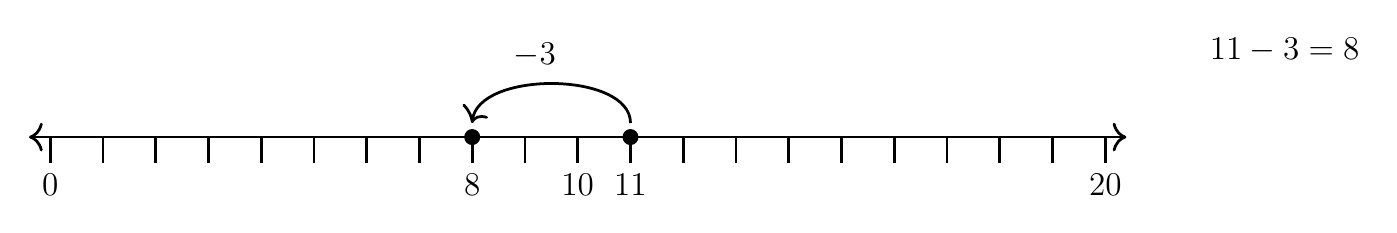
\begin{tikzpicture}[scale=0.67, baseline={([yshift=-1pt]current bounding box.north)}]
    % axis, arrow style to-to
    \draw[{To[scale=1.3]}-{To[scale=1.3]}, line width=1pt] (-0.4, 0) -- (20.4, 0);
    % tick marks
    \foreach \x in {0,1,...,20}
        \draw[shift={(\x,0)},color=black, line width=1pt] (0pt,-14pt) -- (0pt,0pt);
    % numbers along each axis
    \foreach \x in  {0,10,20}
        \draw[shift={(\x,-0.8)},color=black] node[font=\large,text height=12pt] {$\x$};
    \draw[shift={(11,-0.8)},color=black] node[font=\large,text height=12pt] {$11$};
    \draw[shift={(8,-0.8)},color=black] node[font=\large,text height=12pt] {$8$};
    % dots
    \filldraw[black] (11,0) circle (4pt) node[above,yshift=-2pt] (a) {};
    \filldraw[black] (8,0) circle (4pt) node[above,yshift=-2pt] (b) {};
    % arrow
    \draw[-{To[scale=1.3, bend]},line width=1pt, color=black] (a.north)  .. controls  +(north:\jumpheight mm) and +(north:\jumpheight mm) .. node[above=2pt,xshift=-6pt,font=\large,text height=10pt] {$-3$} (b.north); % for addition
    % equation at right end
    \node [font=\large, anchor=east] at (25.0,1.65) {$11-3 = 8$};
\end{tikzpicture}
\end{equation}
\vspace{-2pt}\begin{equation}
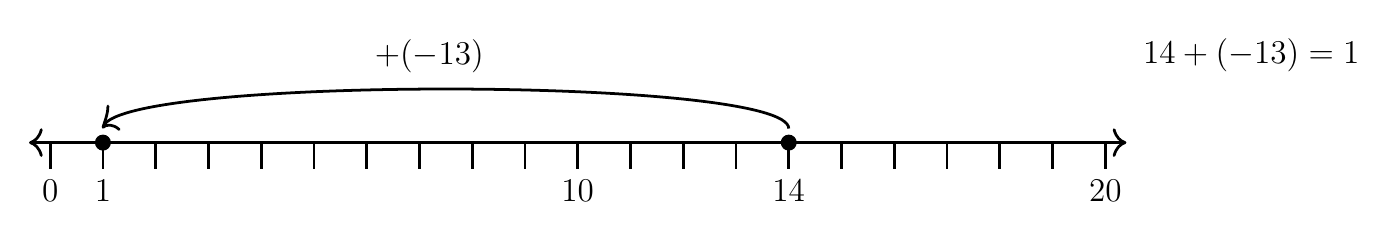
\begin{tikzpicture}[scale=0.67, baseline={([yshift=-1pt]current bounding box.north)}]
    % axis, arrow style to-to
    \draw[{To[scale=1.3]}-{To[scale=1.3]}, line width=1pt] (-0.4, 0) -- (20.4, 0);
    % tick marks
    \foreach \x in {0,1,...,20}
        \draw[shift={(\x,0)},color=black, line width=1pt] (0pt,-14pt) -- (0pt,0pt);
    % numbers along each axis
    \foreach \x in  {0,10,20}
        \draw[shift={(\x,-0.8)},color=black] node[font=\large,text height=12pt] {$\x$};
    \draw[shift={(14,-0.8)},color=black] node[font=\large,text height=12pt] {$14$};
    \draw[shift={(1,-0.8)},color=black] node[font=\large,text height=12pt] {$1$};
    % dots
    \filldraw[black] (14,0) circle (4pt) node[above,yshift=-2pt] (a) {};
    \filldraw[black] (1,0) circle (4pt) node[above,yshift=-2pt] (b) {};
    % arrow
    \draw[-{To[scale=1.3, bend]},line width=1pt, color=black] (a.north)  .. controls  +(north:\jumpheight mm) and +(north:\jumpheight mm) .. node[above=2pt,xshift=-6pt,font=\large,text height=10pt] {$+(-13)$} (b.north); % for addition
    % equation at right end
    \node [font=\large, anchor=east] at (25.0,1.65) {$14+(-13) = 1$};
\end{tikzpicture}
\end{equation}
\vspace{-2pt}\pagebreak ~ \newline ~ \newline\begin{equation}
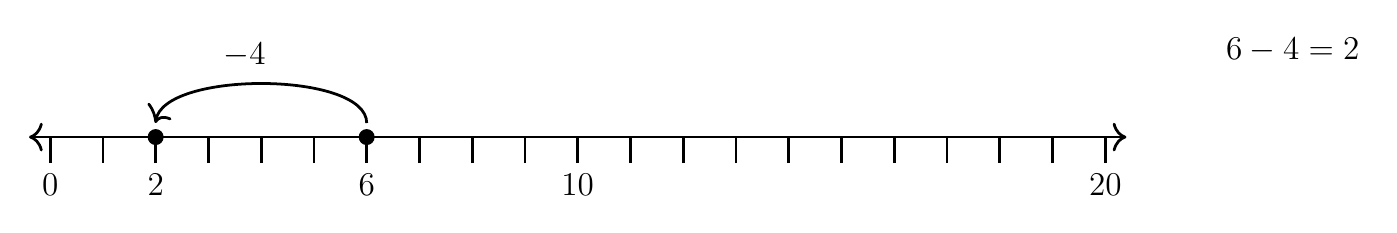
\begin{tikzpicture}[scale=0.67, baseline={([yshift=-1pt]current bounding box.north)}]
    % axis, arrow style to-to
    \draw[{To[scale=1.3]}-{To[scale=1.3]}, line width=1pt] (-0.4, 0) -- (20.4, 0);
    % tick marks
    \foreach \x in {0,1,...,20}
        \draw[shift={(\x,0)},color=black, line width=1pt] (0pt,-14pt) -- (0pt,0pt);
    % numbers along each axis
    \foreach \x in  {0,10,20}
        \draw[shift={(\x,-0.8)},color=black] node[font=\large,text height=12pt] {$\x$};
    \draw[shift={(6,-0.8)},color=black] node[font=\large,text height=12pt] {$6$};
    \draw[shift={(2,-0.8)},color=black] node[font=\large,text height=12pt] {$2$};
    % dots
    \filldraw[black] (6,0) circle (4pt) node[above,yshift=-2pt] (a) {};
    \filldraw[black] (2,0) circle (4pt) node[above,yshift=-2pt] (b) {};
    % arrow
    \draw[-{To[scale=1.3, bend]},line width=1pt, color=black] (a.north)  .. controls  +(north:\jumpheight mm) and +(north:\jumpheight mm) .. node[above=2pt,xshift=-6pt,font=\large,text height=10pt] {$-4$} (b.north); % for addition
    % equation at right end
    \node [font=\large, anchor=east] at (25.0,1.65) {$6-4 = 2$};
\end{tikzpicture}
\end{equation}
\vspace{-2pt}\begin{equation}
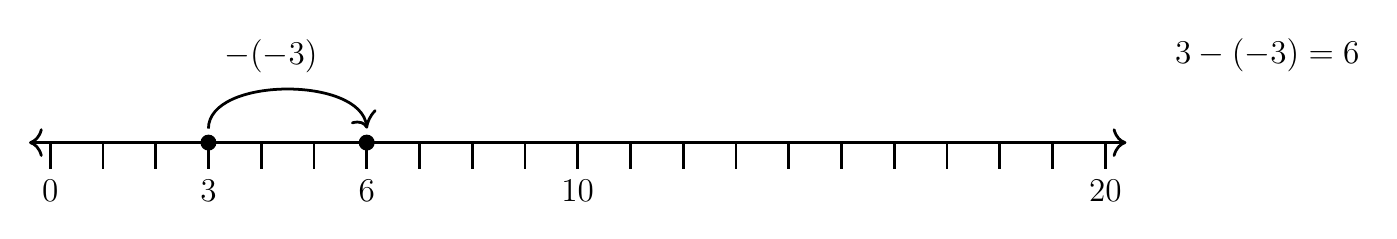
\begin{tikzpicture}[scale=0.67, baseline={([yshift=-1pt]current bounding box.north)}]
    % axis, arrow style to-to
    \draw[{To[scale=1.3]}-{To[scale=1.3]}, line width=1pt] (-0.4, 0) -- (20.4, 0);
    % tick marks
    \foreach \x in {0,1,...,20}
        \draw[shift={(\x,0)},color=black, line width=1pt] (0pt,-14pt) -- (0pt,0pt);
    % numbers along each axis
    \foreach \x in  {0,10,20}
        \draw[shift={(\x,-0.8)},color=black] node[font=\large,text height=12pt] {$\x$};
    \draw[shift={(3,-0.8)},color=black] node[font=\large,text height=12pt] {$3$};
    \draw[shift={(6,-0.8)},color=black] node[font=\large,text height=12pt] {$6$};
    % dots
    \filldraw[black] (3,0) circle (4pt) node[above,yshift=-2pt] (a) {};
    \filldraw[black] (6,0) circle (4pt) node[above,yshift=-2pt] (b) {};
    % arrow
    \draw[-{To[scale=1.3, bend]},line width=1pt, color=black] (a.north)  .. controls  +(north:\jumpheight mm) and +(north:\jumpheight mm) .. node[above=2pt,xshift=-6pt,font=\large,text height=10pt] {$-(-3)$} (b.north); % for addition
    % equation at right end
    \node [font=\large, anchor=east] at (25.0,1.65) {$3-(-3) = 6$};
\end{tikzpicture}
\end{equation}
\vspace{-2pt}\begin{equation}
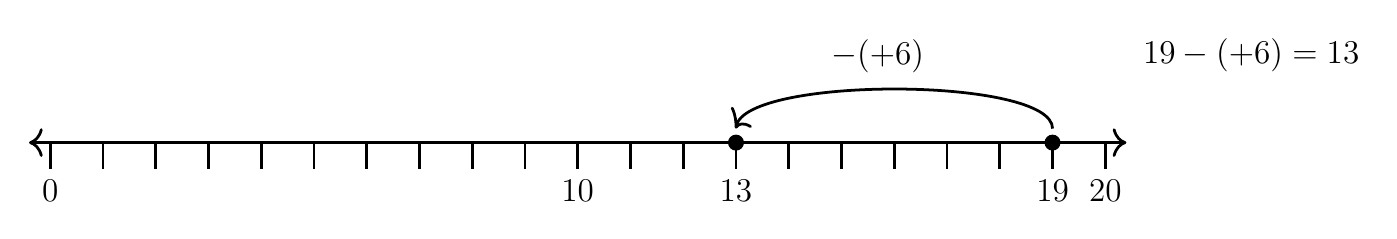
\begin{tikzpicture}[scale=0.67, baseline={([yshift=-1pt]current bounding box.north)}]
    % axis, arrow style to-to
    \draw[{To[scale=1.3]}-{To[scale=1.3]}, line width=1pt] (-0.4, 0) -- (20.4, 0);
    % tick marks
    \foreach \x in {0,1,...,20}
        \draw[shift={(\x,0)},color=black, line width=1pt] (0pt,-14pt) -- (0pt,0pt);
    % numbers along each axis
    \foreach \x in  {0,10,20}
        \draw[shift={(\x,-0.8)},color=black] node[font=\large,text height=12pt] {$\x$};
    \draw[shift={(19,-0.8)},color=black] node[font=\large,text height=12pt] {$19$};
    \draw[shift={(13,-0.8)},color=black] node[font=\large,text height=12pt] {$13$};
    % dots
    \filldraw[black] (19,0) circle (4pt) node[above,yshift=-2pt] (a) {};
    \filldraw[black] (13,0) circle (4pt) node[above,yshift=-2pt] (b) {};
    % arrow
    \draw[-{To[scale=1.3, bend]},line width=1pt, color=black] (a.north)  .. controls  +(north:\jumpheight mm) and +(north:\jumpheight mm) .. node[above=2pt,xshift=-6pt,font=\large,text height=10pt] {$-(+6)$} (b.north); % for addition
    % equation at right end
    \node [font=\large, anchor=east] at (25.0,1.65) {$19-(+6) = 13$};
\end{tikzpicture}
\end{equation}
\vspace{-2pt}\begin{equation}
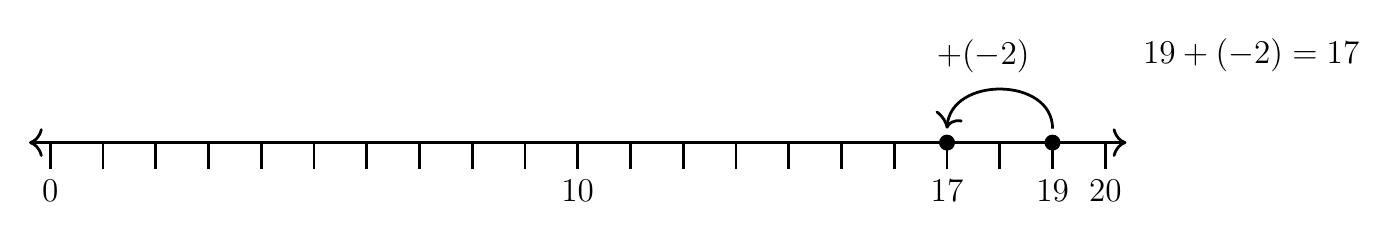
\begin{tikzpicture}[scale=0.67, baseline={([yshift=-1pt]current bounding box.north)}]
    % axis, arrow style to-to
    \draw[{To[scale=1.3]}-{To[scale=1.3]}, line width=1pt] (-0.4, 0) -- (20.4, 0);
    % tick marks
    \foreach \x in {0,1,...,20}
        \draw[shift={(\x,0)},color=black, line width=1pt] (0pt,-14pt) -- (0pt,0pt);
    % numbers along each axis
    \foreach \x in  {0,10,20}
        \draw[shift={(\x,-0.8)},color=black] node[font=\large,text height=12pt] {$\x$};
    \draw[shift={(19,-0.8)},color=black] node[font=\large,text height=12pt] {$19$};
    \draw[shift={(17,-0.8)},color=black] node[font=\large,text height=12pt] {$17$};
    % dots
    \filldraw[black] (19,0) circle (4pt) node[above,yshift=-2pt] (a) {};
    \filldraw[black] (17,0) circle (4pt) node[above,yshift=-2pt] (b) {};
    % arrow
    \draw[-{To[scale=1.3, bend]},line width=1pt, color=black] (a.north)  .. controls  +(north:\jumpheight mm) and +(north:\jumpheight mm) .. node[above=2pt,xshift=-6pt,font=\large,text height=10pt] {$+(-2)$} (b.north); % for addition
    % equation at right end
    \node [font=\large, anchor=east] at (25.0,1.65) {$19+(-2) = 17$};
\end{tikzpicture}
\end{equation}
\vspace{-2pt}\begin{equation}
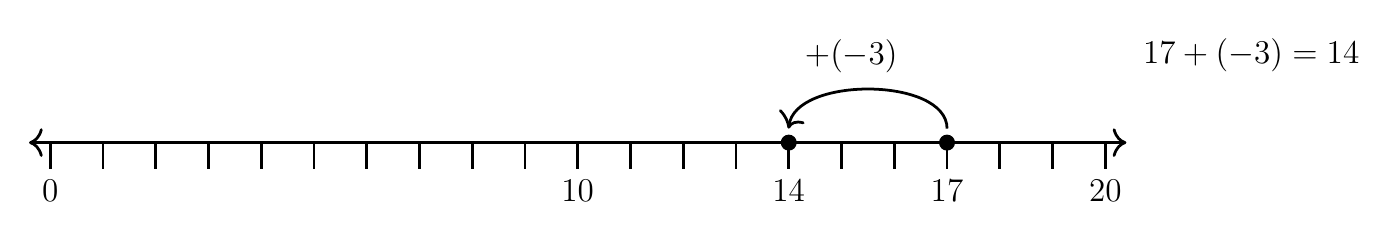
\begin{tikzpicture}[scale=0.67, baseline={([yshift=-1pt]current bounding box.north)}]
    % axis, arrow style to-to
    \draw[{To[scale=1.3]}-{To[scale=1.3]}, line width=1pt] (-0.4, 0) -- (20.4, 0);
    % tick marks
    \foreach \x in {0,1,...,20}
        \draw[shift={(\x,0)},color=black, line width=1pt] (0pt,-14pt) -- (0pt,0pt);
    % numbers along each axis
    \foreach \x in  {0,10,20}
        \draw[shift={(\x,-0.8)},color=black] node[font=\large,text height=12pt] {$\x$};
    \draw[shift={(17,-0.8)},color=black] node[font=\large,text height=12pt] {$17$};
    \draw[shift={(14,-0.8)},color=black] node[font=\large,text height=12pt] {$14$};
    % dots
    \filldraw[black] (17,0) circle (4pt) node[above,yshift=-2pt] (a) {};
    \filldraw[black] (14,0) circle (4pt) node[above,yshift=-2pt] (b) {};
    % arrow
    \draw[-{To[scale=1.3, bend]},line width=1pt, color=black] (a.north)  .. controls  +(north:\jumpheight mm) and +(north:\jumpheight mm) .. node[above=2pt,xshift=-6pt,font=\large,text height=10pt] {$+(-3)$} (b.north); % for addition
    % equation at right end
    \node [font=\large, anchor=east] at (25.0,1.65) {$17+(-3) = 14$};
\end{tikzpicture}
\end{equation}
\vspace{-2pt}\begin{equation}
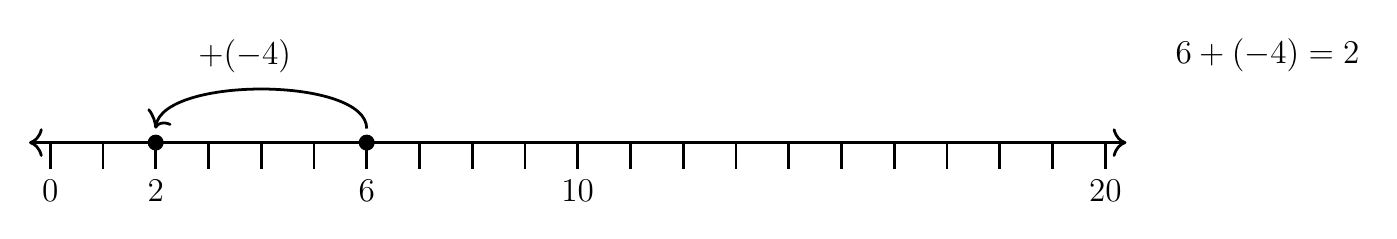
\begin{tikzpicture}[scale=0.67, baseline={([yshift=-1pt]current bounding box.north)}]
    % axis, arrow style to-to
    \draw[{To[scale=1.3]}-{To[scale=1.3]}, line width=1pt] (-0.4, 0) -- (20.4, 0);
    % tick marks
    \foreach \x in {0,1,...,20}
        \draw[shift={(\x,0)},color=black, line width=1pt] (0pt,-14pt) -- (0pt,0pt);
    % numbers along each axis
    \foreach \x in  {0,10,20}
        \draw[shift={(\x,-0.8)},color=black] node[font=\large,text height=12pt] {$\x$};
    \draw[shift={(6,-0.8)},color=black] node[font=\large,text height=12pt] {$6$};
    \draw[shift={(2,-0.8)},color=black] node[font=\large,text height=12pt] {$2$};
    % dots
    \filldraw[black] (6,0) circle (4pt) node[above,yshift=-2pt] (a) {};
    \filldraw[black] (2,0) circle (4pt) node[above,yshift=-2pt] (b) {};
    % arrow
    \draw[-{To[scale=1.3, bend]},line width=1pt, color=black] (a.north)  .. controls  +(north:\jumpheight mm) and +(north:\jumpheight mm) .. node[above=2pt,xshift=-6pt,font=\large,text height=10pt] {$+(-4)$} (b.north); % for addition
    % equation at right end
    \node [font=\large, anchor=east] at (25.0,1.65) {$6+(-4) = 2$};
\end{tikzpicture}
\end{equation}
\vspace{-2pt}\begin{equation}
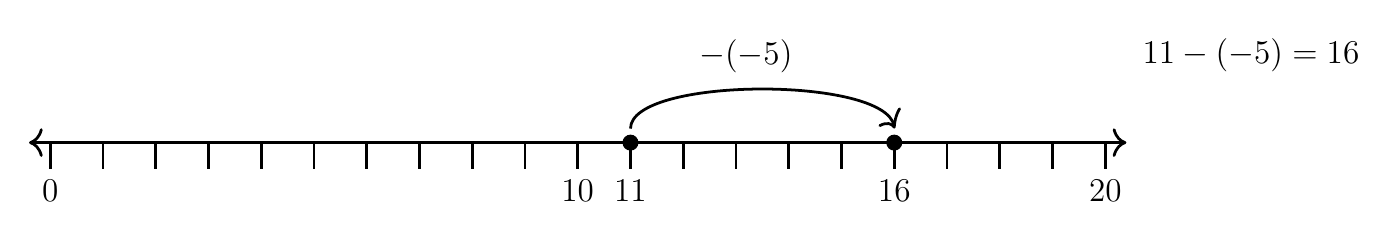
\begin{tikzpicture}[scale=0.67, baseline={([yshift=-1pt]current bounding box.north)}]
    % axis, arrow style to-to
    \draw[{To[scale=1.3]}-{To[scale=1.3]}, line width=1pt] (-0.4, 0) -- (20.4, 0);
    % tick marks
    \foreach \x in {0,1,...,20}
        \draw[shift={(\x,0)},color=black, line width=1pt] (0pt,-14pt) -- (0pt,0pt);
    % numbers along each axis
    \foreach \x in  {0,10,20}
        \draw[shift={(\x,-0.8)},color=black] node[font=\large,text height=12pt] {$\x$};
    \draw[shift={(11,-0.8)},color=black] node[font=\large,text height=12pt] {$11$};
    \draw[shift={(16,-0.8)},color=black] node[font=\large,text height=12pt] {$16$};
    % dots
    \filldraw[black] (11,0) circle (4pt) node[above,yshift=-2pt] (a) {};
    \filldraw[black] (16,0) circle (4pt) node[above,yshift=-2pt] (b) {};
    % arrow
    \draw[-{To[scale=1.3, bend]},line width=1pt, color=black] (a.north)  .. controls  +(north:\jumpheight mm) and +(north:\jumpheight mm) .. node[above=2pt,xshift=-6pt,font=\large,text height=10pt] {$-(-5)$} (b.north); % for addition
    % equation at right end
    \node [font=\large, anchor=east] at (25.0,1.65) {$11-(-5) = 16$};
\end{tikzpicture}
\end{equation}
\vspace{-2pt}\begin{equation}
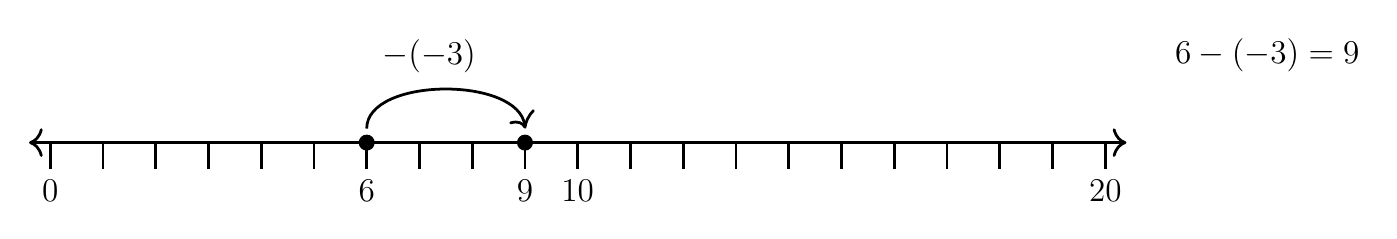
\begin{tikzpicture}[scale=0.67, baseline={([yshift=-1pt]current bounding box.north)}]
    % axis, arrow style to-to
    \draw[{To[scale=1.3]}-{To[scale=1.3]}, line width=1pt] (-0.4, 0) -- (20.4, 0);
    % tick marks
    \foreach \x in {0,1,...,20}
        \draw[shift={(\x,0)},color=black, line width=1pt] (0pt,-14pt) -- (0pt,0pt);
    % numbers along each axis
    \foreach \x in  {0,10,20}
        \draw[shift={(\x,-0.8)},color=black] node[font=\large,text height=12pt] {$\x$};
    \draw[shift={(6,-0.8)},color=black] node[font=\large,text height=12pt] {$6$};
    \draw[shift={(9,-0.8)},color=black] node[font=\large,text height=12pt] {$9$};
    % dots
    \filldraw[black] (6,0) circle (4pt) node[above,yshift=-2pt] (a) {};
    \filldraw[black] (9,0) circle (4pt) node[above,yshift=-2pt] (b) {};
    % arrow
    \draw[-{To[scale=1.3, bend]},line width=1pt, color=black] (a.north)  .. controls  +(north:\jumpheight mm) and +(north:\jumpheight mm) .. node[above=2pt,xshift=-6pt,font=\large,text height=10pt] {$-(-3)$} (b.north); % for addition
    % equation at right end
    \node [font=\large, anchor=east] at (25.0,1.65) {$6-(-3) = 9$};
\end{tikzpicture}
\end{equation}
\vspace{-2pt}
\end{document}


